\chapter{Versuchsdokumentation}
\label{app:ch:versuche}

\chapter{SCRUM Board per Sprint}

\begin{landscape}
	\section*{Sprint01 Review und Sprint02 Planning}
	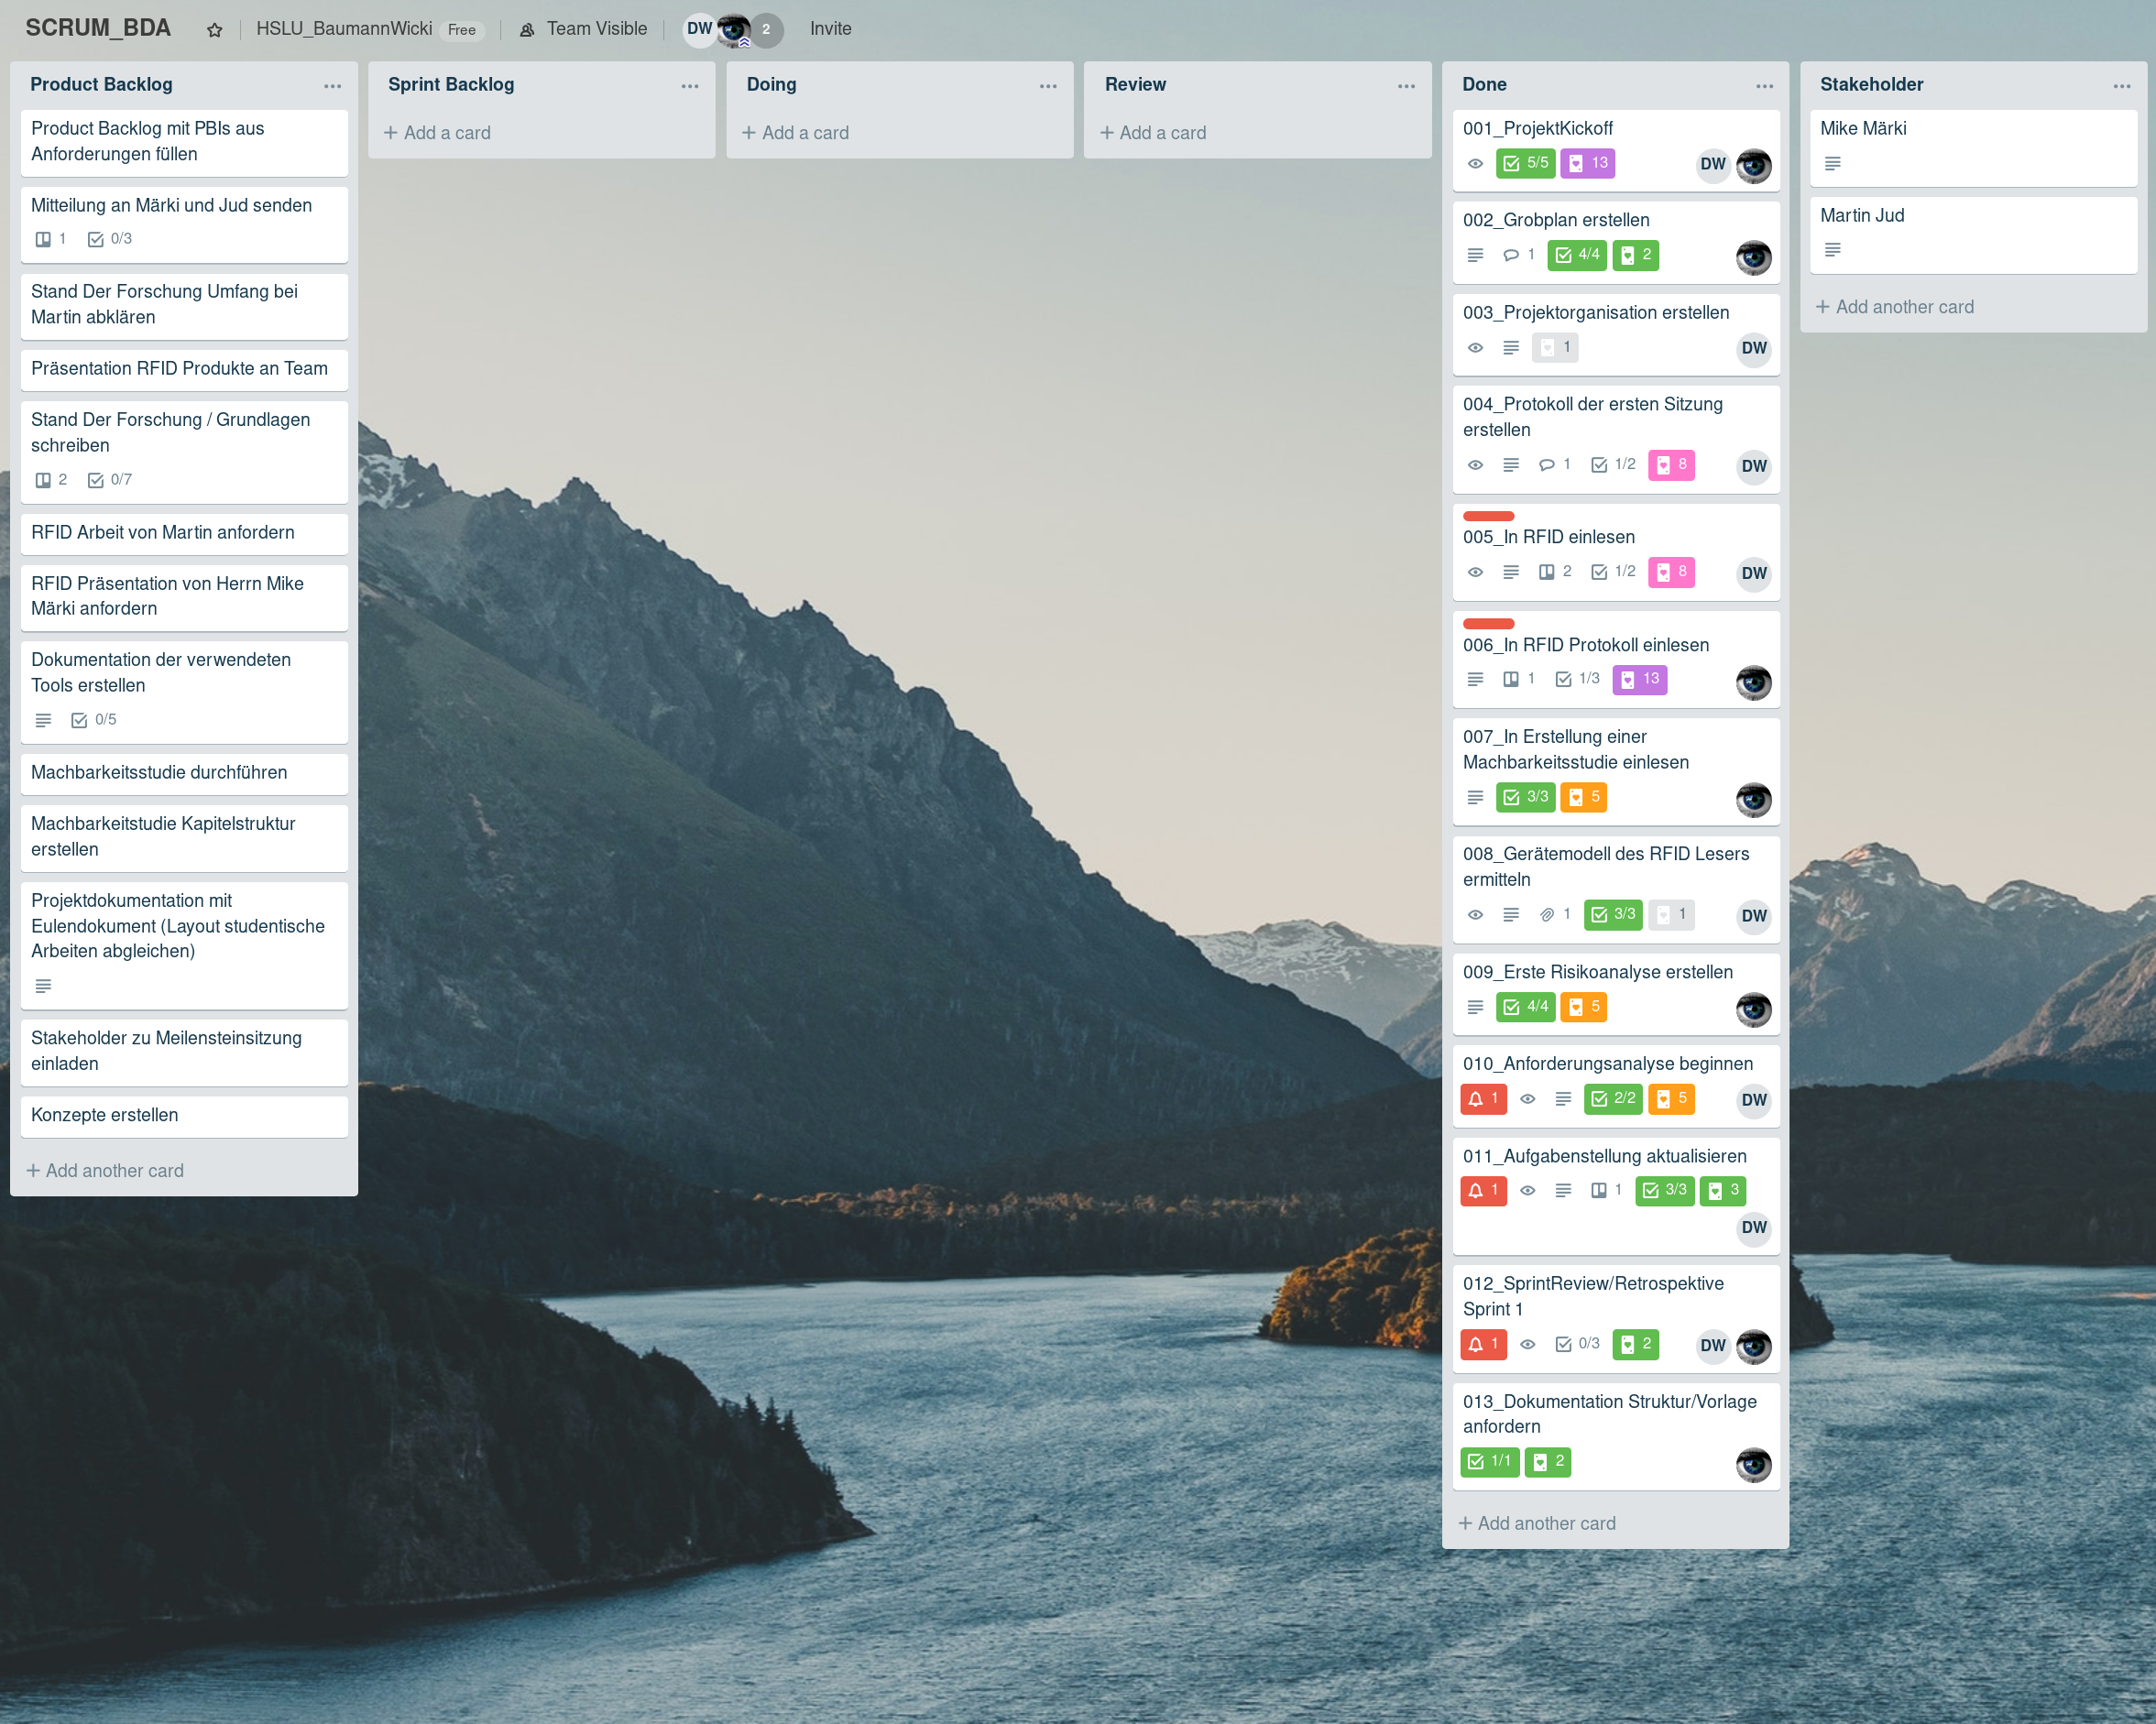
\includegraphics[height=0.9\textheight,keepaspectratio]{Sprint01_Review_Sprint02_Planning.png}
\end{landscape}

\newpage
\section*{Sprint02 Review}
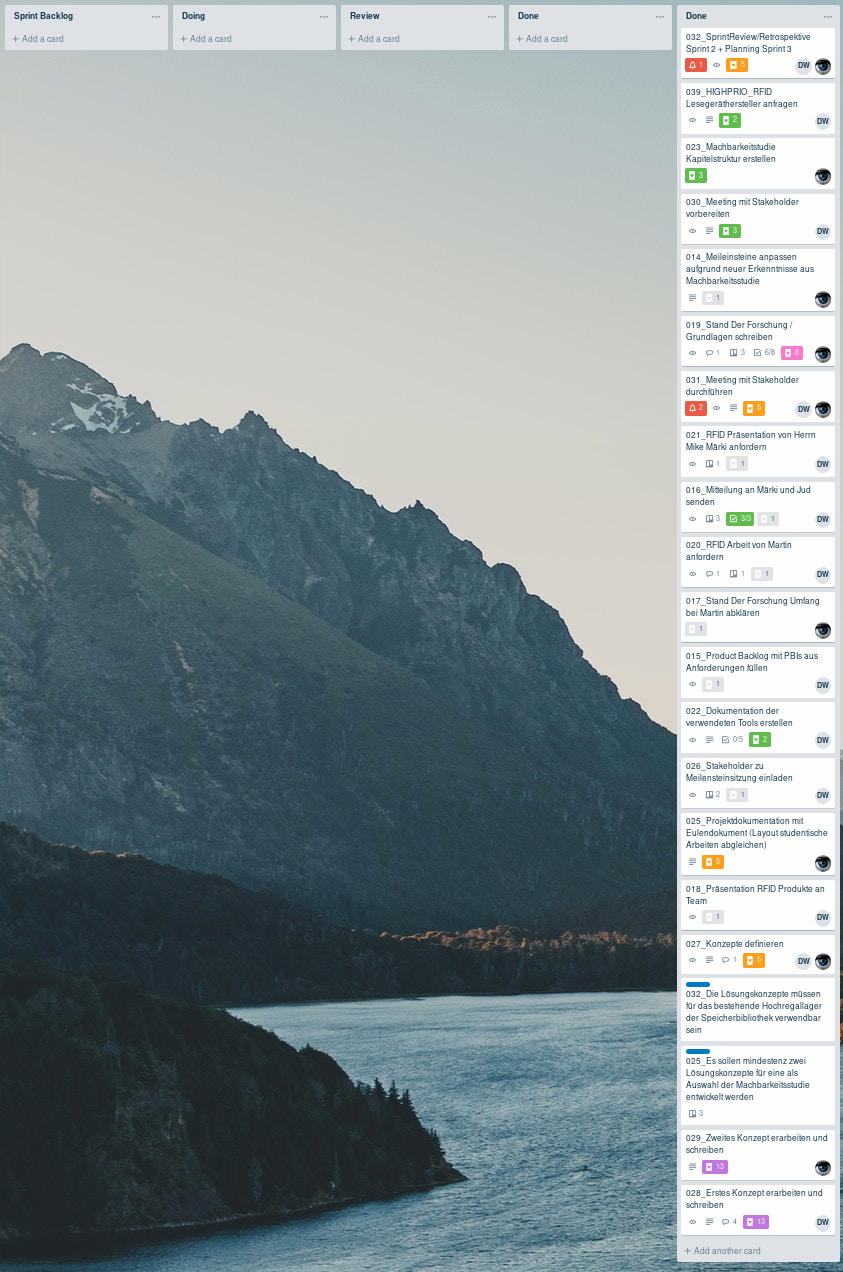
\includegraphics[height=0.9\textheight,keepaspectratio]{Sprint02_Review.png}

\newpage
\begin{landscape}
	\section*{Sprint03 Planning}
	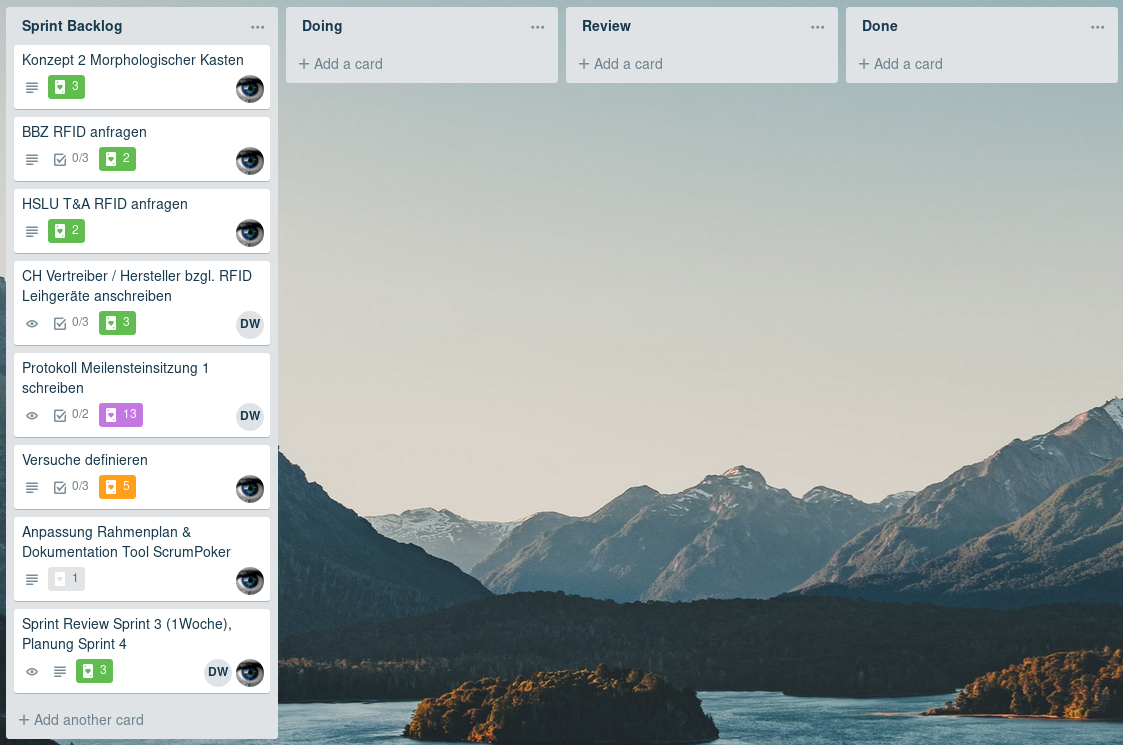
\includegraphics[height=0.9\textheight,keepaspectratio]{Sprint03_Planning.png}
\end{landscape}

\newpage
\section*{Sprint03 Review}
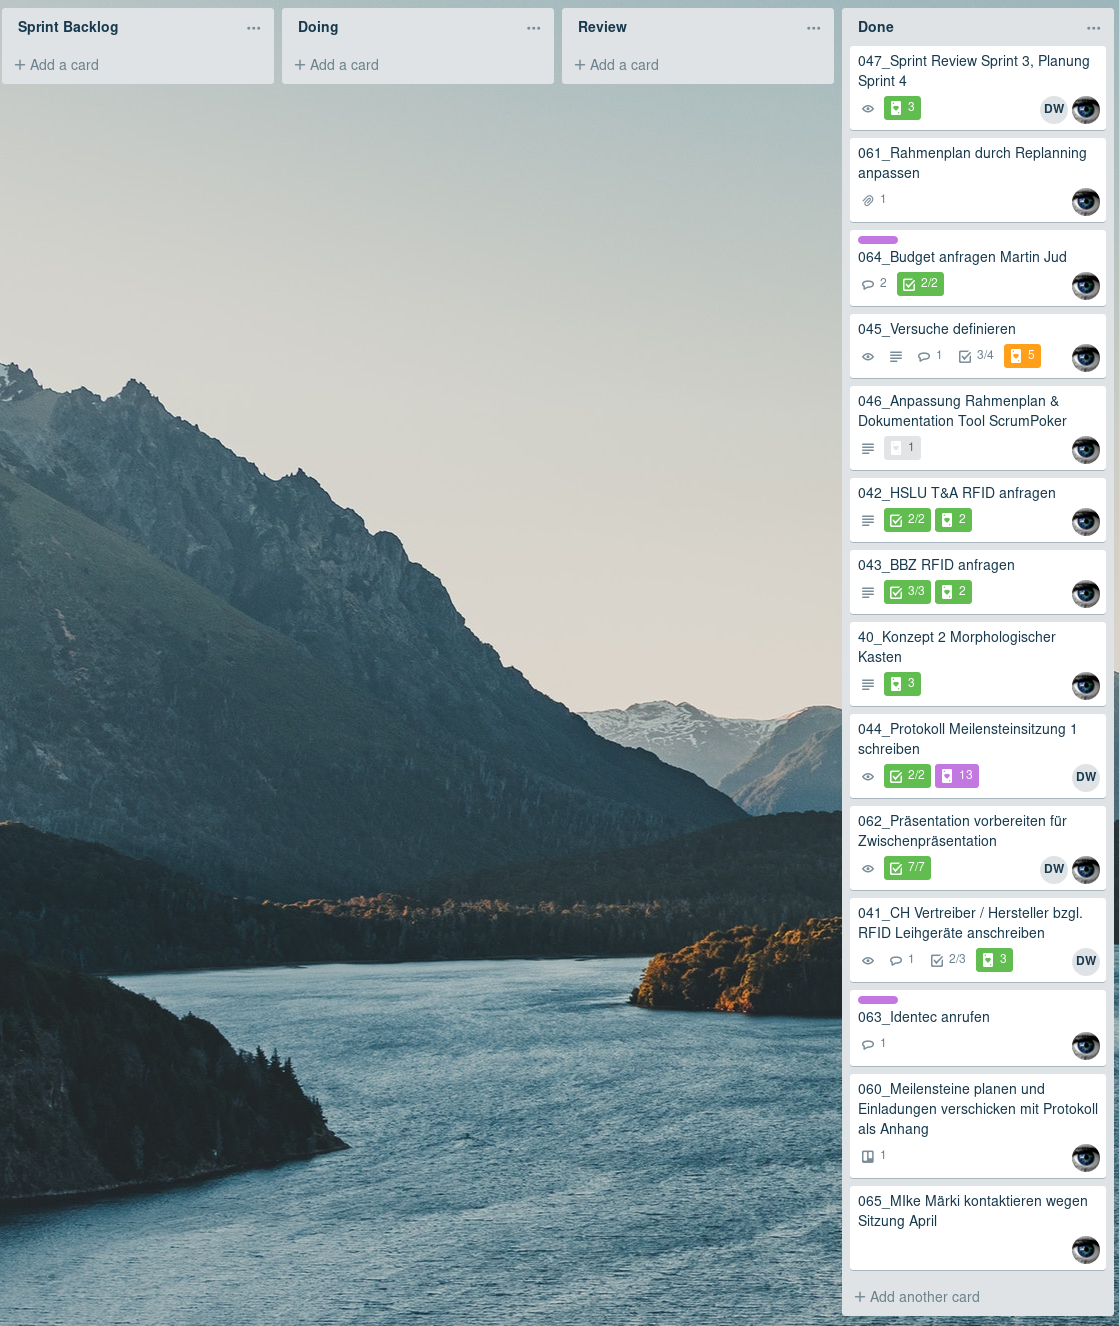
\includegraphics[width=\linewidth,keepaspectratio]{Sprint03_Review.png}

\newpage
\begin{landscape}
	\section*{Sprint04 Review}
	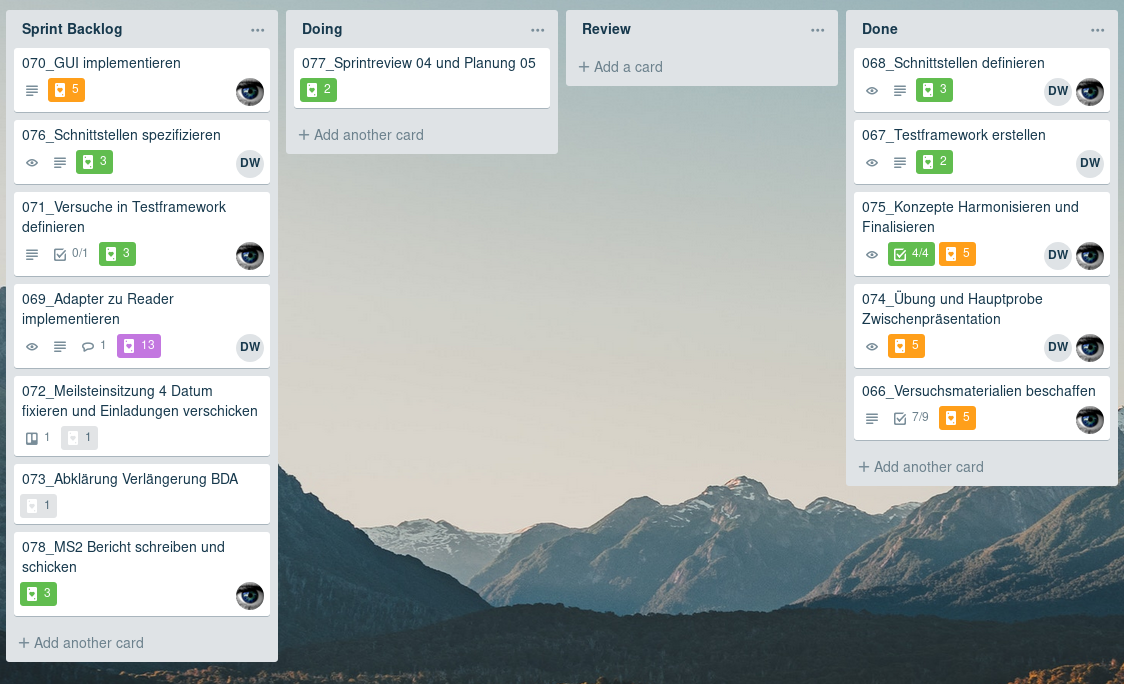
\includegraphics[height=0.9\textheight,keepaspectratio]{Sprint04_Review.png}
\end{landscape}

\newpage
\section*{Sprint05 Planning}
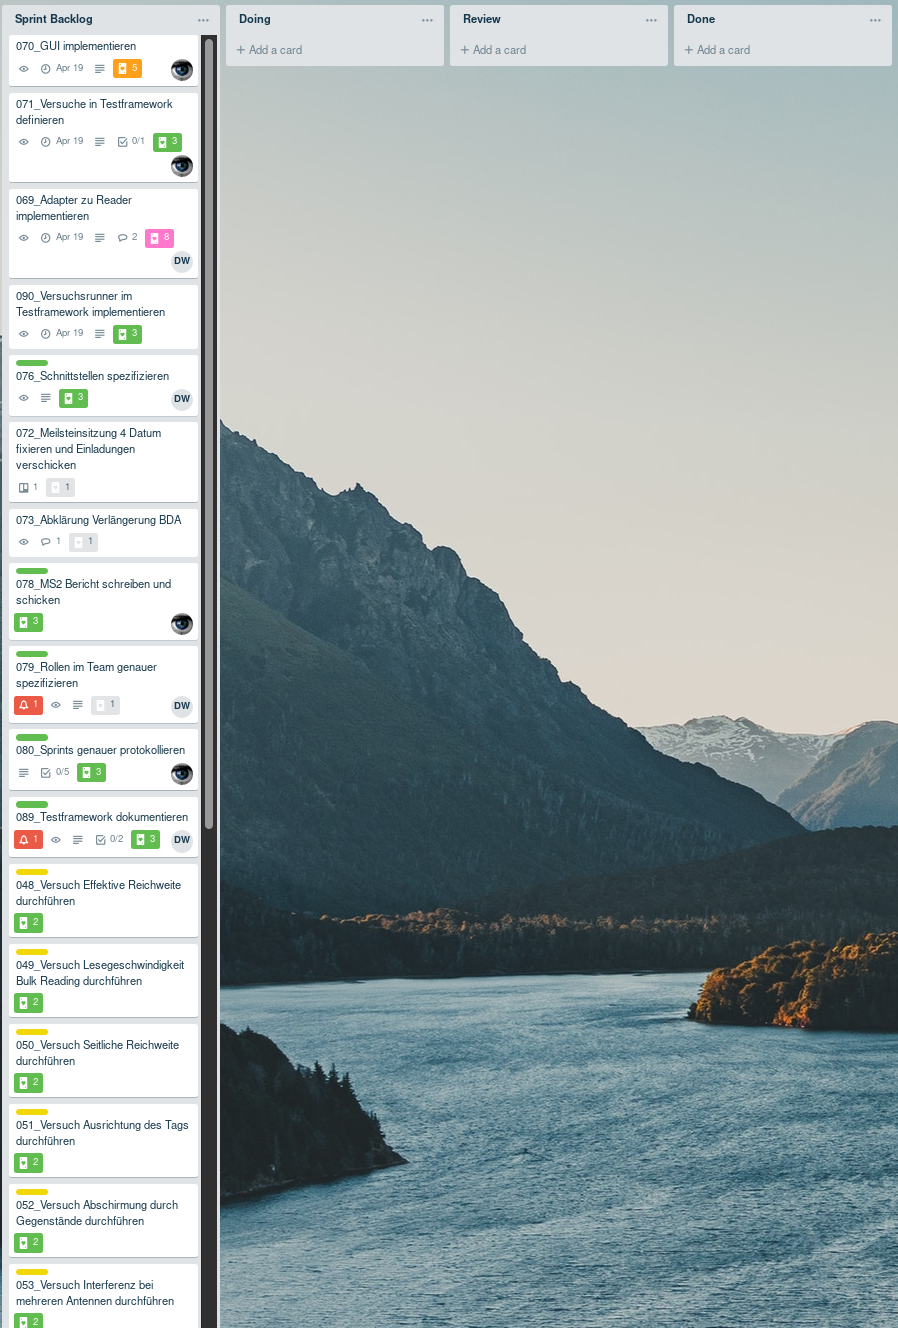
\includegraphics[width=0.9\linewidth,keepaspectratio]{Sprint05_Planning_01.png}
\newpage
\noindent
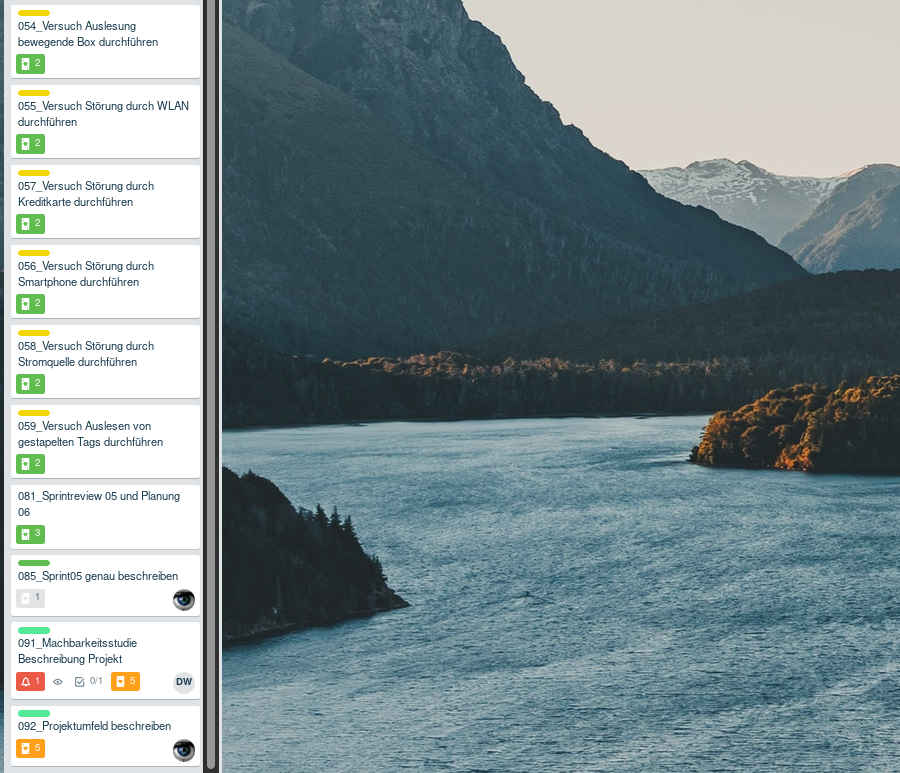
\includegraphics[width=0.9\linewidth,keepaspectratio]{Sprint05_Planning_02.png}

\chapter{Hardware Spezifikation}
\label{app:ch:hardwarespez}
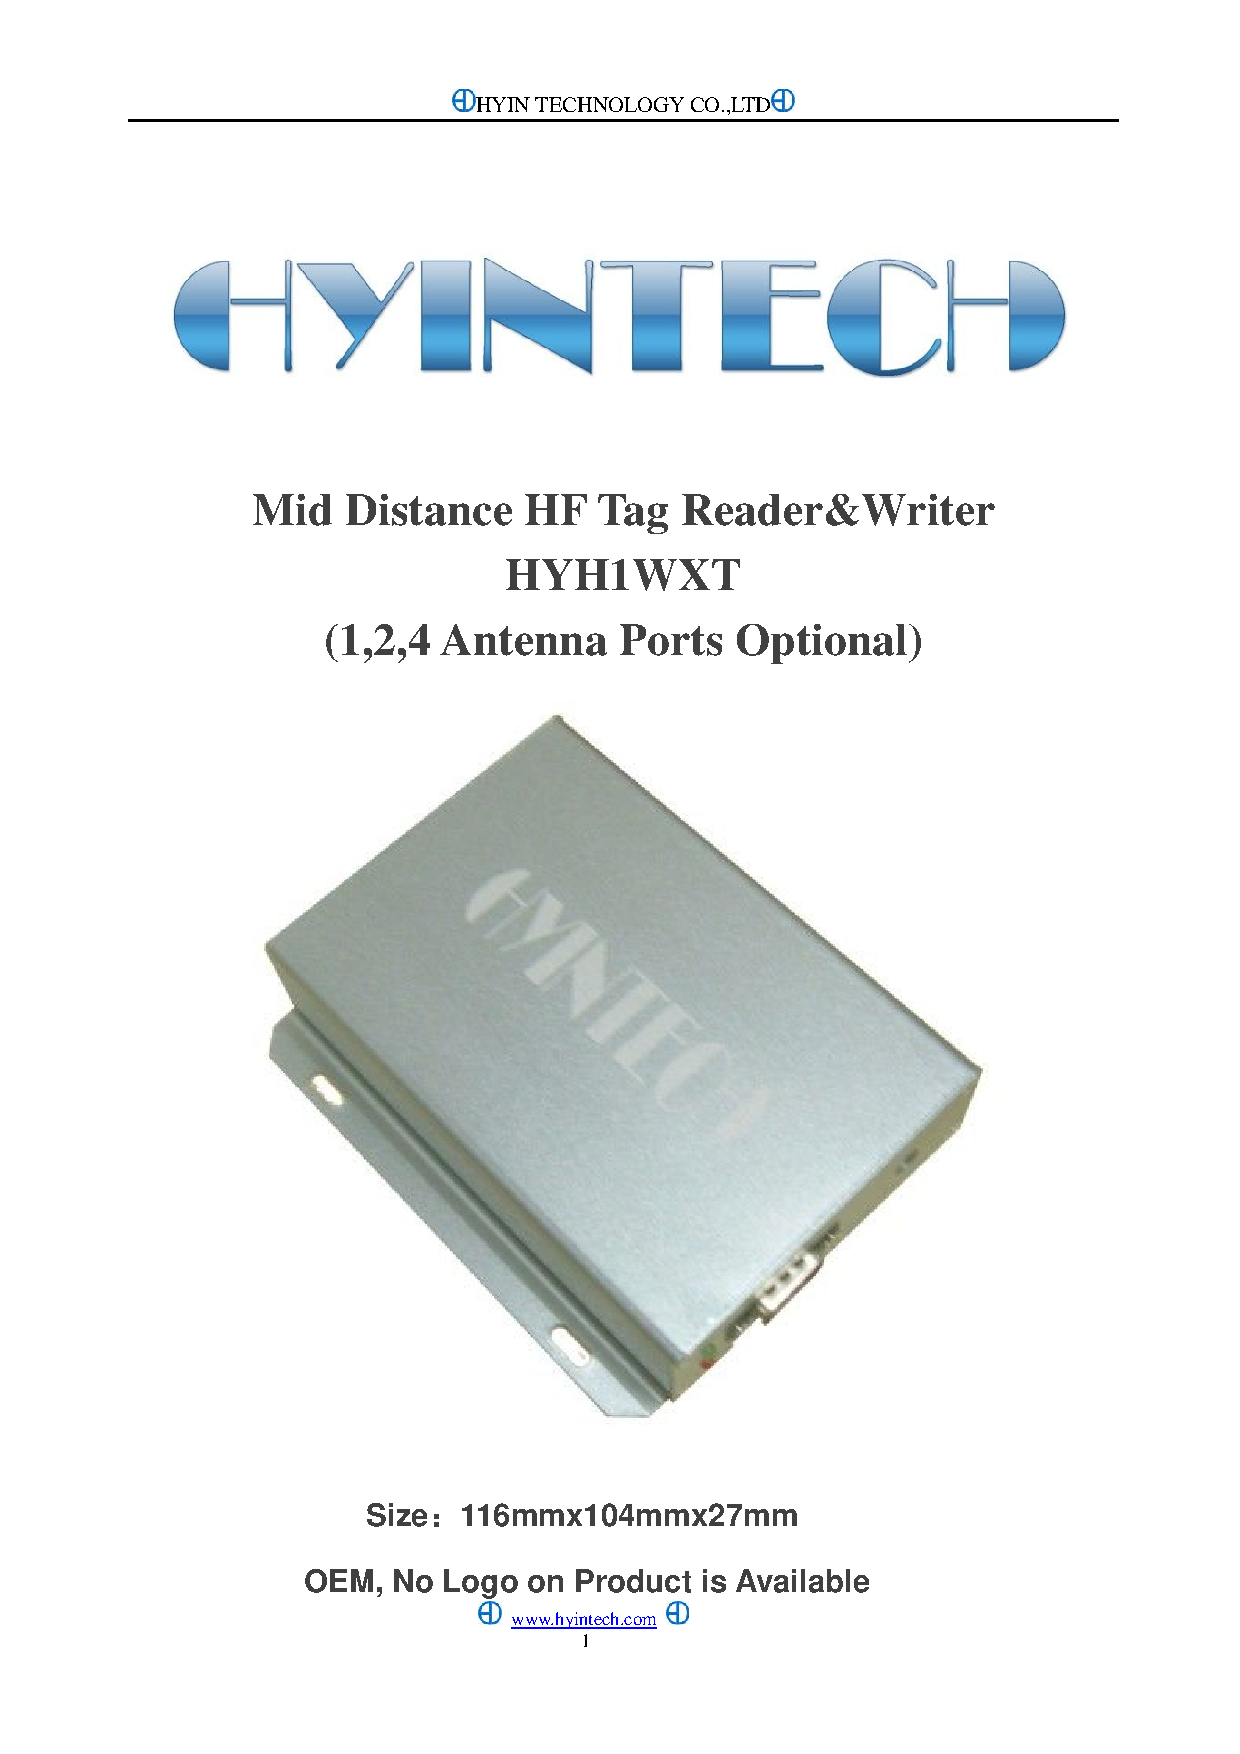
\includepdf[pages=-]{HYH1WXT_Spec_EN}
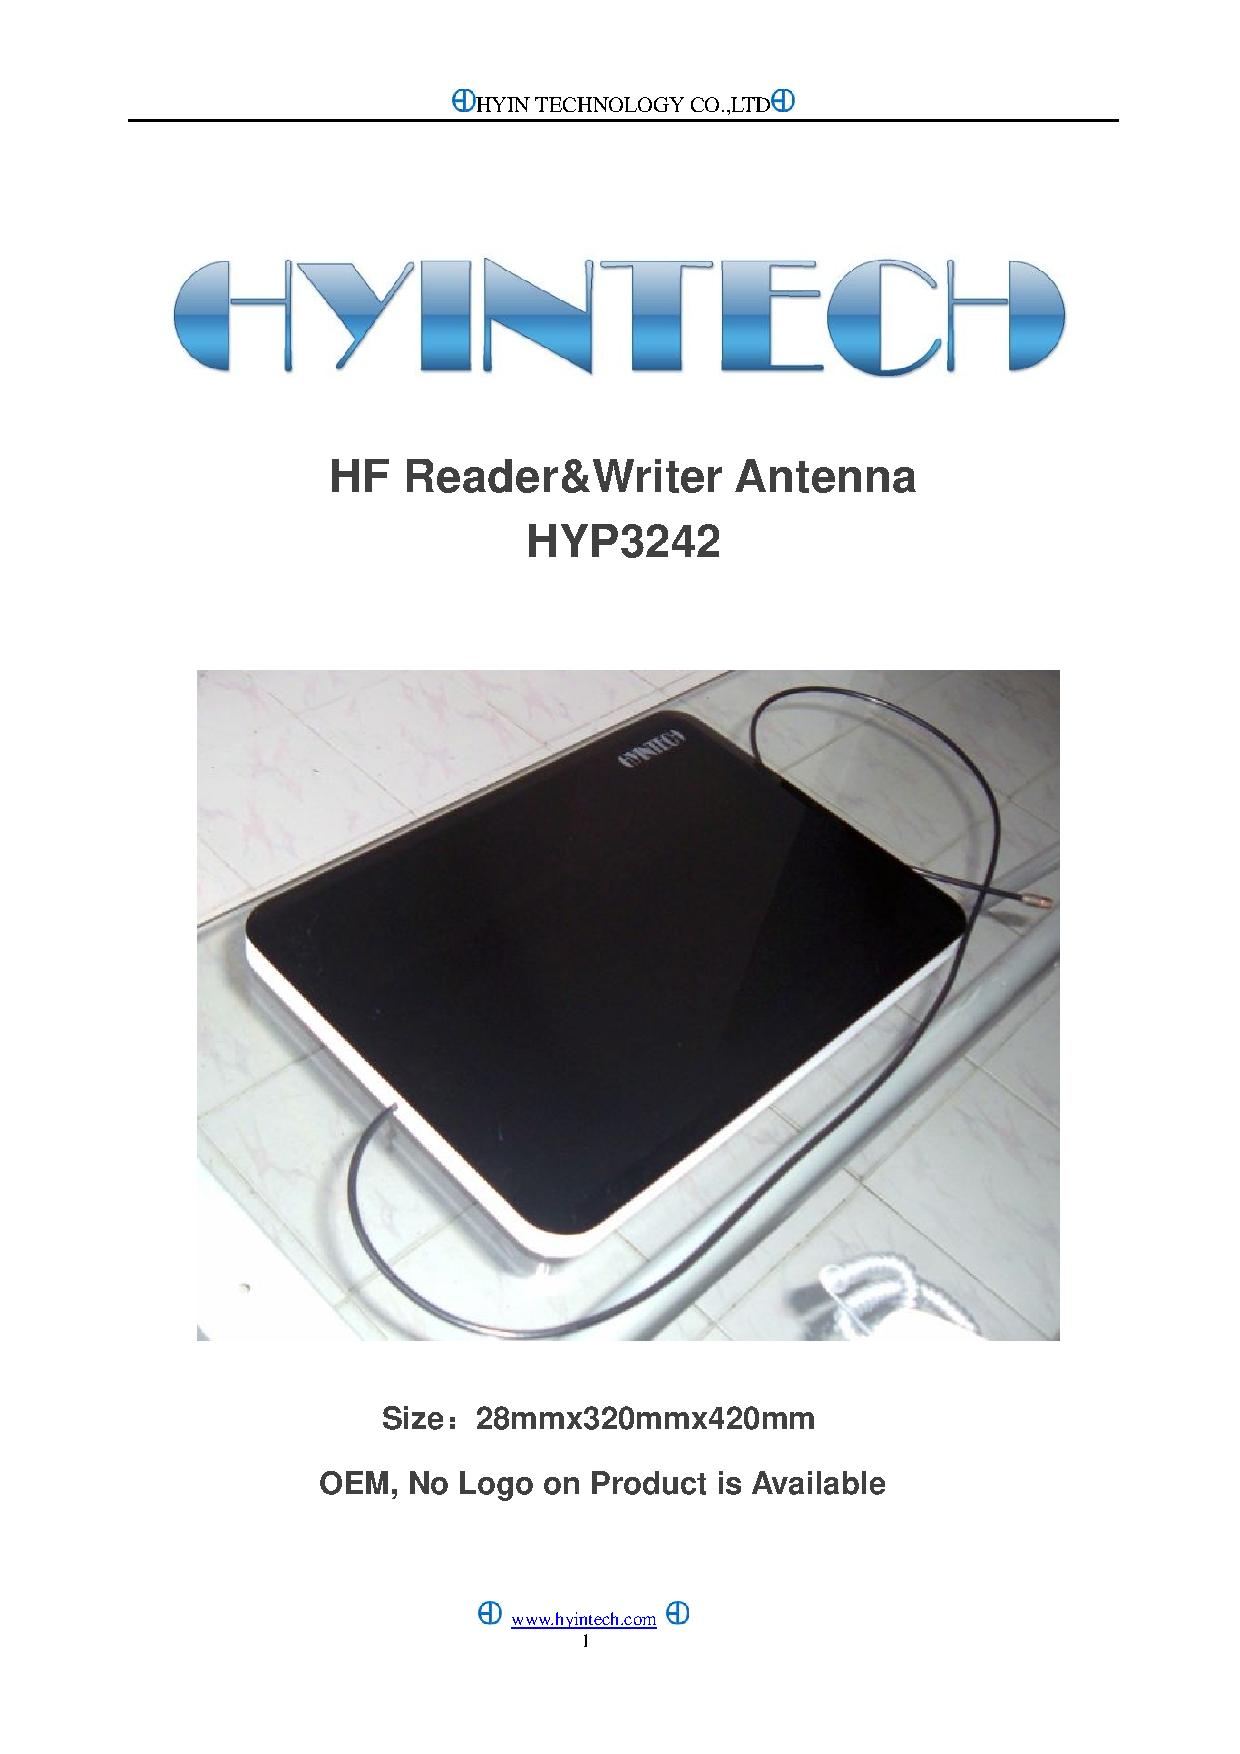
\includepdf[pages=-]{HYP3242_Spec_EN}
\chapter{DLL Spezifikationen Hyientech}
\label{app:ch:dllspezifikation}
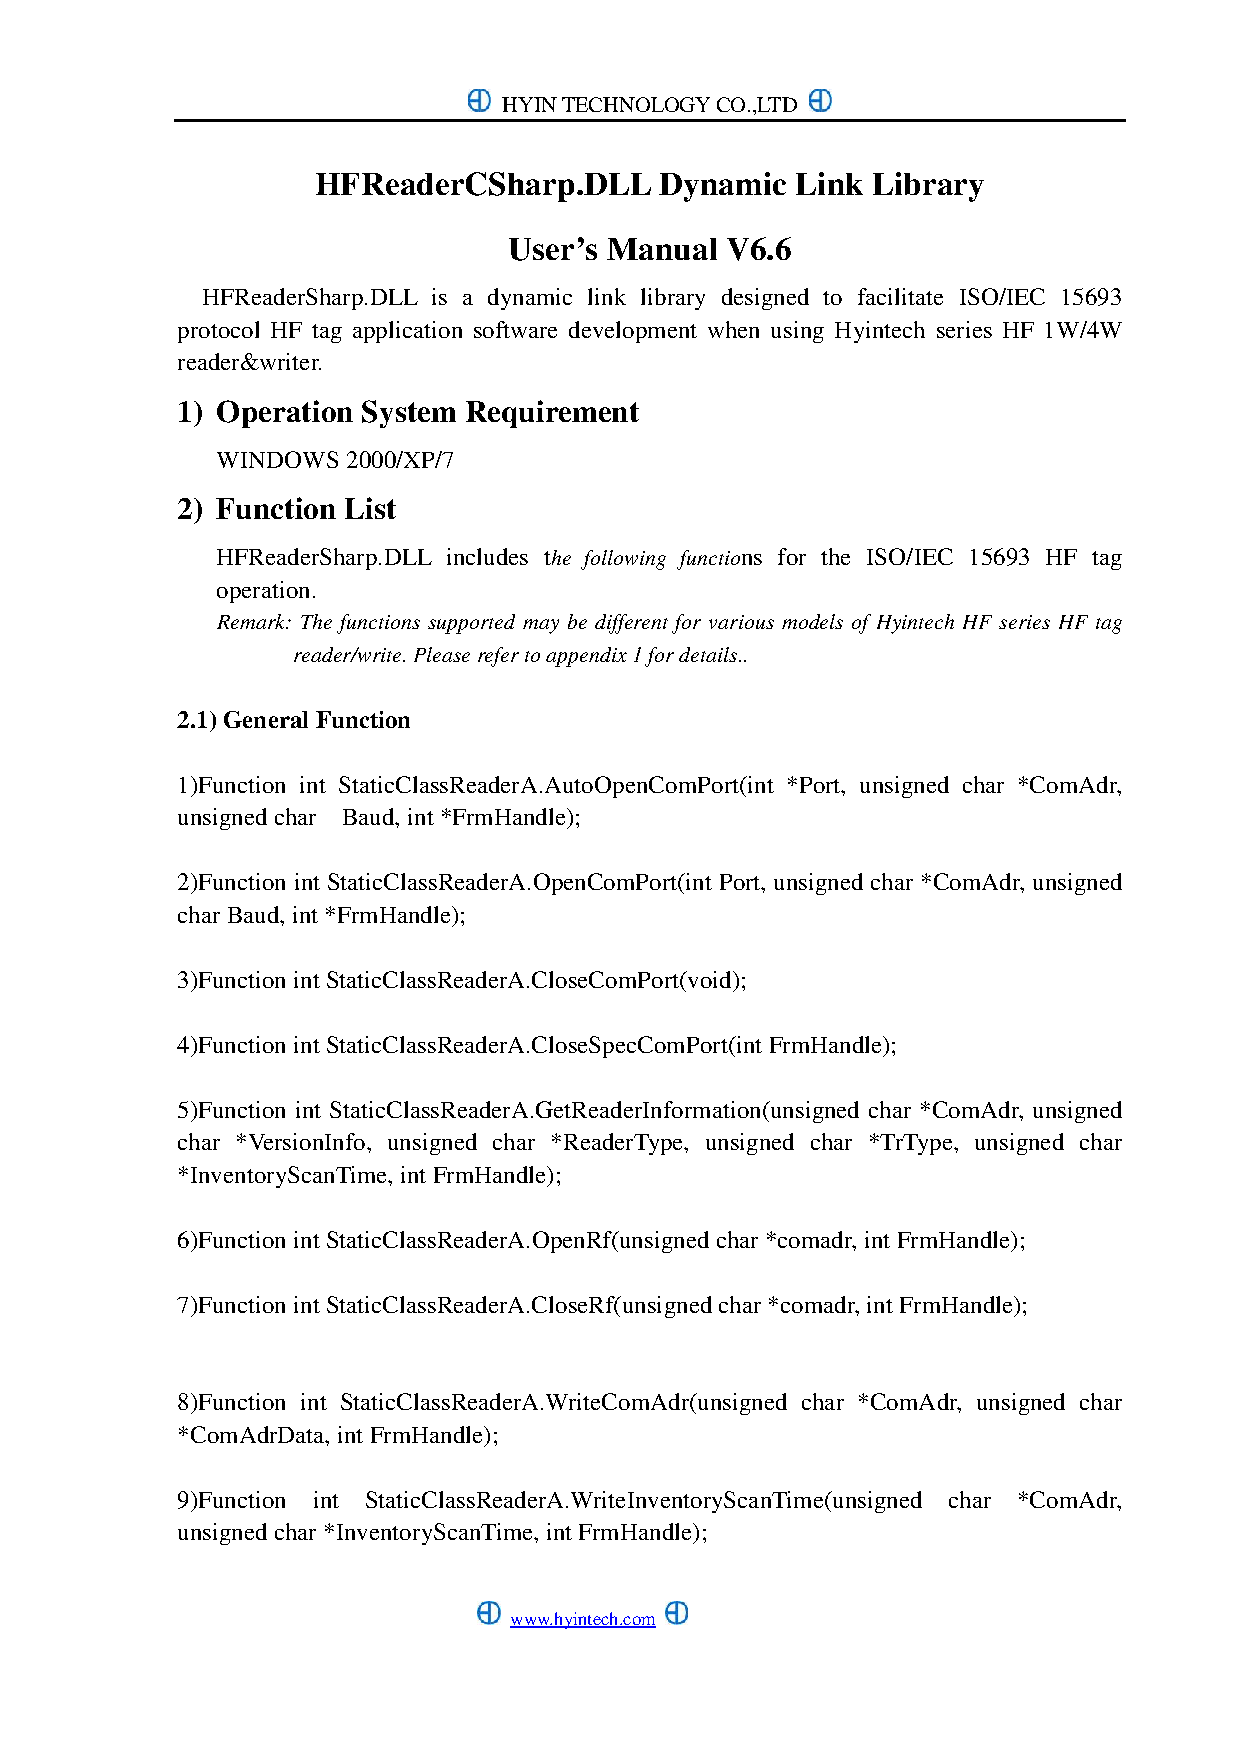
\includepdf[pages=-]{HyientechDLL_Spec}